\documentclass[12pt]{article}
%\renewcommand\normalsize{\fontsize{10pt}{12pt}\selectfont}
\usepackage{graphicx} % Required for inserting images
\usepackage[left=2cm,right=2cm,top=2cm,bottom=1.5cm]{geometry}

\title{Quiz 5}
%\author{Dennis Wilkinson}
\date{due Tuesday April 29}

\begin{document}

\setlength{\parindent}{0pt}
\setlength{\parskip}{3mm}

FS1 Wilkinson Quiz 5, June 5, 2025

\textbf{1.} Consider the circuit below where $V=1$ volt and $R_1=R_2=10$ $\Omega$. Perhaps it is a battery powering two light wired in parallel.
\begin{figure}[h]
    \centering
    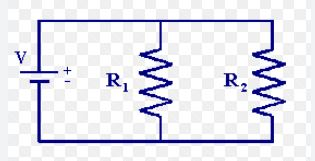
\includegraphics[width=0.3\linewidth]{parallel circuit.JPG}
\end{figure}

\textbf{a.} Find the current in each of the resistors. 

\vspace{1in}

\textbf{b.} Find the power being produced by the battery.

\vspace{1in}

\textbf{c.} If we placed a third identical resistor in parallel with $R_1$ and $R_2$, would the current from the battery increase, decrease, or stay the same? Also, what would happen to the brightness of $R_1$ and $R_2$ (light bulb brightness is proportional to power)? Justify your answers. 

\vspace{1in}

\textbf{2.} A wire is carrying current eastward and there is a magnetic field pointing north. 

\textbf{a.} What direction is the magnetic force on the wire?

\vspace{0.5in}

\textbf{b.} Same question if the wire is running northeast. Also, is the force greater, the same, or less than in part (a)? Why?

\end{document}